% Presenter info: 
% SIGOPS
%
% Use a two-column, 8.5" x 11" document format
% Use a 0.75" margin everywhere
% All fonts MUST be Type 1 or 3 PostScript fornst from the Latin 1 Fontset.
% Do not use TruType, bitmapped, or Ryumin fonts.
% Use 10-point font size.
%

\documentclass{../common/acm}

\usepackage{verbatim,moreverb}
\usepackage{float}
\usepackage{graphicx}

% Needed for LLNL cover page / TID bibliography style
\usepackage{calc}
\usepackage{epsfig}
\usepackage{graphics}
\usepackage{hhline}
\input{pstricks}
\input{pst-node}
\usepackage{chngpage}
% ***************** llnlCoverPage.tex ********************************************************************************
% This file defines the following commands for generating the
% front and back cover pages:
%
%     \makeLLNLCover{UCRL}{Title}{Authors}{Journal}{Date}{hShift}{vShift}
%  and
%     \makeLLNLBackCover
%
% where
%
%  UCRL: The UCRL (6 digit) number (which you probably won't know before the document
%        is released so just make up a number)
%  Title: title of the article
%  Authors: Authors separated by \\
%  Journal: The journal name
%  Date : the date
%  hShift,vShift : horizontal and vertical shifts to apply to the title page to position it correctly (since
%                  the automatic positioning may not work)
%
% Here is an example:
%  \makeLLNLCover{123456}{An adaptive numerical method for high-speed reactive flows}{William D. Henshaw\\%
%   Donald W. Schwendeman}{Journal of Computational Physics}{January 1, 2003}{0in}{0in}
%
% *****************************************************************************************************************
%
\newcommand{\setPageForLLNLCover}[2]{%
\newlength{\textwidthOld}%
\setlength{\textwidthOld}{\textwidth}%
\newlength{\textheightOld}%
\setlength{\textheightOld}{\textheight}%
\newlength{\topmarginOld}%
\setlength{\topmarginOld}{\topmargin}%
\newlength{\textwidthNew}%
\setlength{\textwidthNew}{6.5in}%
\newlength{\textheightNew}%
\setlength{\textheightNew}{9.5in}%
\newlength{\oddsidemarginNew}%
\newlength{\topmarginNew}%
\setlength{\oddsidemarginNew}{(\paperwidth-\textwidthNew)/2 - 1in + #1}%
\setlength{\topmarginNew}{(\paperheight-\textheightNew -\headheight-\headsep-\footskip)/2 - 1in +1.cm + #2}%
\newlength{\oddsidemarginOld}%
\setlength{\oddsidemarginOld}{\oddsidemargin}%
\changepage{\textheightNew-\textheightOld}{\textwidthNew-\textwidthOld}{\oddsidemarginNew-\oddsidemarginOld}{\oddsidemarginNew-\oddsidemarginOld}{}{\topmarginNew-\topmarginOld}{}{}{}%
}%
\newcommand{\setPageForLLNLBackCover}{%
\changepage{\textheightNew-\textheightOld}{\textwidthNew-\textwidthOld}{\oddsidemarginNew-\oddsidemarginOld}{\oddsidemarginNew-\oddsidemarginOld}{}{\topmarginNew-\topmarginOld}{}{}{}%
}%
\newcommand{\resetPageFromLLNLCover}{%
\changepage{-\textheightNew+\textheightOld}{-\textwidthNew+\textwidthOld}{-\oddsidemarginNew+\oddsidemarginOld}{-\oddsidemarginNew+\oddsidemarginOld}{}{-\topmarginNew+\topmarginOld}{}{}{}%
}%
% *************************************************************************************


% *************************************************************************************
\newcommand{\makeLLNLCover}[7]{%
\setPageForLLNLCover{#6}{#7}%
\thispagestyle{empty}% no number of this page
\newcommand{\logoWidth}{1.65in}%
\psset{xunit=1.cm,yunit=1.cm,runit=1.cm}%
\begin{pspicture}(0,0)(17,24.)
% turn on the grid for placement
% \psgrid[subgriddiv=2]
\rput(2.3,12.5){
\epsfig{file=../common/Logo_for_papers.ps,width=\logoWidth}}
\rput(11.2,23.){\parbox{12.0cm}{\large\bf%
\begin{flushright}
% jg - just pass in full UCRL string
%Preprint \\
%UCRL-JC-#1
#1
\end{flushright}
}}
\rput(10.5,18){\parbox{12.0cm}{%\sffamily\bfseries\Huge\noindent%
\fontsize{24.88}{30pt}\usefont{OT1}{cmss}{bx}{n}
\begin{flushleft}
#2
\end{flushleft}
}}
\rput(10.5,13.){\parbox{12.0cm}{%\sffamily\LARGE\noindent%
\fontsize{17.28}{18pt}\usefont{OT1}{cmss}{m}{sl}
\begin{flushleft}
#3
\end{flushleft}
}}
\rput(10.5,9.5){\parbox{12.0cm}{% \sffamily\large\noindent%
\fontsize{14}{16pt}\usefont{OT1}{cmss}{m}{n}
This article was submitted to #4
}}
\rput(10.5,7.5){\parbox{12.0cm}{% \sffamily\bfseries\LARGE\noindent%
\fontsize{20.74}{22pt}\usefont{OT1}{cmss}{bx}{n}
\begin{flushleft}
#5
\end{flushleft}
}}
% \rput[l](4,6.375){\psframebox{\parbox{2.5cm}{\bf%
% \begin{flushleft}
% Lawrence\\
% Livermore\\
% National\\
% Laboratory
% \end{flushleft}
% }}}
\rput(10.5,-1.){\parbox{12.0cm}{%
Approved for public release; further dissemination unlimited}}
\end{pspicture}
% }
%
\clearpage
% -------------- back of front cover -------------------------
\changetext{.625in}{}{}{}{}
\thispagestyle{empty}% no number of this page
\vglue5\baselineskip
\begin{center}
{\bf DISCLAIMER}
\end{center}
\noindent
% jg - updated disclaimer for report format
This document was prepared as an account of work sponsored by an
agency of the United States Government.  Neither the United States
Government nor the University of California nor any of their
employees, makes any warranty, express or implied, or assumes any
legal liability or responsibility for the accuracy, completeness, or
usefulness of any information, apparatus, product, or process
disclosed, or represents that its use would not infringe privately
owned rights. Reference herein to any specific commercial product,
process, or service by trade name, trademark, manufacturer, or
otherwise, does not necessarily constitute or imply its endorsement,
recommendation, or favoring by the United States Government or the
University of California.  The views and opinions of authors expressed
herein do not necessarily state or reflect those of the United States
Government or the University of California, and shall not be used for
advertising or product endorsement purposes.
\vskip2\baselineskip
\noindent
This work was performed under the auspices of the U. S. Department of
Energy by the University of California, Lawrence Livermore National
Laboratory under Contract No. W-7405-Eng-48.
\vskip1\baselineskip
\vfill
\clearpage
\changetext{-.625in}{}{}{}{}
\resetPageFromLLNLCover
\setcounter{page}{1}
% -----------------------------------------------------------------------------------
}
% *************************************************************************************


% *************************************************************************************
\newcommand{\makeLLNLBackCover}{%
\clearpage
\setPageForLLNLBackCover
% jg - suppress printing of essentially blank page here
%\changetext{.625in}{}{}{}{}
%\thispagestyle{empty}% no number of this page
\ \
%\vfill
%\begin{center}
%Approved for public release; further dissemination unlimited
%\end{center}
%\clearpage
%\clearpage
%\changetext{-.625in}{}{}{}{}
% ---------------------------------------------------------------------------
\thispagestyle{empty}% no number of this page
\renewcommand{\logoWidth}{10.in}
% \vglue\vShift
% \hglue\hShift
\begin{pspicture}(0,0)(17,24.)
% turn on the grid for placement
% \psgrid[subgriddiv=2]
\rput{90}(2.3,12.5){
\epsfig{file=../common/Rule_and_address.ps,width=\logoWidth}}
% \rput*[l]{90}(5.5,0){\psframebox{\parbox{8.0cm}{\large%
% \begin{flushleft}
% University of California\\
% Lawrence Livermore National Laboratory\\
% Technical Information Department\\
% Livermore, CA 94551
% \end{flushleft}
% }}}
\end{pspicture}
% \setlength{\textwidth}{4.in}      % page width
% \setlength{\textheight}{8.in}    % page height
\clearpage
\resetPageFromLLNLCover
% -----------------------------------------------------------------------------------
}
% *************************************************************************************






% Uncomment for DRAFT "watermark"
%\usepackage{draftcopy}

% Times font as default roman
\renewcommand{\sfdefault}{phv}
\renewcommand{\rmdefault}{ptm}
%\renewcommand{\ttdefault}{pcr}
%\usepackage{times}
\renewcommand{\labelitemi}{$\bullet$}

\setlength{\oddsidemargin}{-0.25in}
\setlength{\evensidemargin}{-0.25in}
\setlength{\topmargin}{-0.25in} % was{-0.75in}
\setlength{\headsep}{0.5in}
\setlength{\footskip}{24.0pt}
\setlength{\textheight}{9.5in}
\setlength{\columnwidth}{3.32in}
\setlength{\textwidth}{7.0in}
\setlength{\columnsep}{0.30in}
\setlength{\columnseprule}{0.0pt}

% couple of macros for the title page and document
\def\ctit{Scalable Resource Management with SLURM}
\def\ucrl{UCRL-JC-TBD}
\def\auth{Morris Jette}
\def\pubdate{January 23, 2006}
\def\journal{Operating Systems Reviews}

\begin{document}

% make the cover page
%\makeLLNLCover{\ucrl}{\ctit}{\auth}{\journal}{\pubdate}{0in}{0in}

\title{\ctit}
\numberofauthors{1}
\author{
\alignauthor Morris Jette\\
	\affaddr{Lawrence Livermore National Laboratory}\\
	\affaddr{Livermore, CA, USA}\\
	\email{jette1@llnl.gov}
}

\maketitle
\begin{abstract}
While the increase in performance of individual computer 
processors through the years has been impressive, the demand
for compute resources has grown even more rapidly. 
This demand has been met over the past couple of decades by 
turning to parallel computing. 
While operating systems, compilers, libraries, and a wide 
variety of tools exist to make effective use of independent 
computers, a new class of tools is required to effectively 
utilize a parallel computer. 
One important tool is the resource manager, which can be viewed 
as the "glue" to run applications on the parallel computer. 
One very popular resource manager is the Simple Linux
Utility for Resource Management (SLURM, 
http://www.llnl.gov/linux/slurm). 
SLURM performs resource management on about 1000 parallel 
computers around the world, including many of the largest 
systems. 
This paper will describe resource management scalability 
issues and SLURM's implementation.
\end{abstract}


\section{Introduction}

Executing a parallel program on a cluster involves several 
steps. First resources (cores, memory, nodes, etc.) suitable 
for running the program must be identified. These resources 
are then typically dedicated to the program. In some 
cases, the computer's network/interconnect must be 
configured for the program's use. The program's tasks
are initiated on the allocated resources. The input and 
output for all of these tasks must be processed. 
Upon the program termination, it's allocated resources 
are released for use by other programs. 
All of these operations are straightforward, but performing 
resource management on clusters containing thousands of 
nodes and over 130,000 processor cores requires more 
than a high degree of parallelism.
In many respects, data management and fault-tolerance issues
are paramount.

SLURM is a resource manager jointly developed by Lawrence 
Livermore National Laboratory (LLNL), 
Hewlett-Packard, and Linux NetworX
~\cite{SLURM2003,Yoo2003,SlurmWeb}.
SLURM's general characteristics include:

\begin{itemize}
\item {\tt Simplicity}: SLURM is simple enough to allow motivated 
end users to understand its source code and add functionality. 
It supports only a few simple scheduling algorithms, 
but relies upon an external scheduler for sophisticated
workload prioritization.

\item {\tt Open Source}: SLURM is available to everyone and 
will remain free.
Its source code is distributed under the GNU General Public
License
~\cite{GPL2002}.

\item {\tt Portability}: SLURM is written in the C language, 
with a GNU {\em autoconf} configuration engine.
SLURM has a fully functional skeleton of functionality with a
wide assortment of plugins available for customization. 
A total of 30 different plugins are available and provide a 
great deal of flexibility in configuring SLURM using a 
building block approach.

\item {\tt Scalability}: SLURM is designed for scalability to clusters 
of thousands of nodes. Time to fully execute (allocate, launch
tasks, process I/O, and deallocate resources) a simple program
is only 2 seconds for 4,800 tasks on 2,400 nodes. Clusters 
containing up to 16,384 nodes have been emulated with highly 
scalable performance. 

\item {\tt Fault Tolerance}: SLURM can handle a variety of failures
in hardward or the infrastructure without inducing failures in 
the workload.

\item {\tt Security}: SLURM employs crypto technology to authenticate
users to services and services to each other with a variety of options
available through the plugin mechanism.  

\item {\tt System Administrator Friendly}: SLURM utilizes
a simple configuration file and minimizes distributed state.
Its configuration may be changed at any time without impacting running
jobs.  Heterogeneous nodes within a cluster may be easily managed.  SLURM
interfaces are usable by scripts and its behavior is highly deterministic.

\end{itemize}

\section{Architecture}

\begin{figure}[tb]
\centerline{\includegraphics[width=3.32in]{../figures/arch2.eps}}
\caption{\small SLURM architecture}
\label{arch}
\end{figure}

SLURM's commands and daemons are illustrated in Figure~\ref{arch}.
The main SLURM control program, {\tt slurmctld}, orchestrates
activities throughout the cluster. While highly optimized, 
{\tt slurmctld} is best run on a dedicated node of the cluster for optimal performance. 
In addition, SLURM provides the option of running  a backup controller 
on another node for increased fault-tolerance.
Each node in the cluster available for running user applications 
has a relatively small daemon called {\tt slurmd} that monitors
and manages resources and work within that node. 
Several user tools are provided:

\begin{itemize}
\item {\tt scontrol} is a system administrator tool to monitor and change
system configuration

\item {\tt sinfo} reports status and configuration of the nodes and queues

\item {\tt squeue} reports status of jobs

\item {\tt scancel} can signal and/or cancel jobs or job steps

\item {\tt smap} reports node, queue, and job status including 
topological state information

\item {\tt sacct} reports job accounting information

\item {\tt sbcast} copies a file to local file systems on a job's allocated nodes

\item {\tt srun} is used to allocate resources and spawn the job's tasks.
\end{itemize}

\begin{figure}[tcb]
\centerline{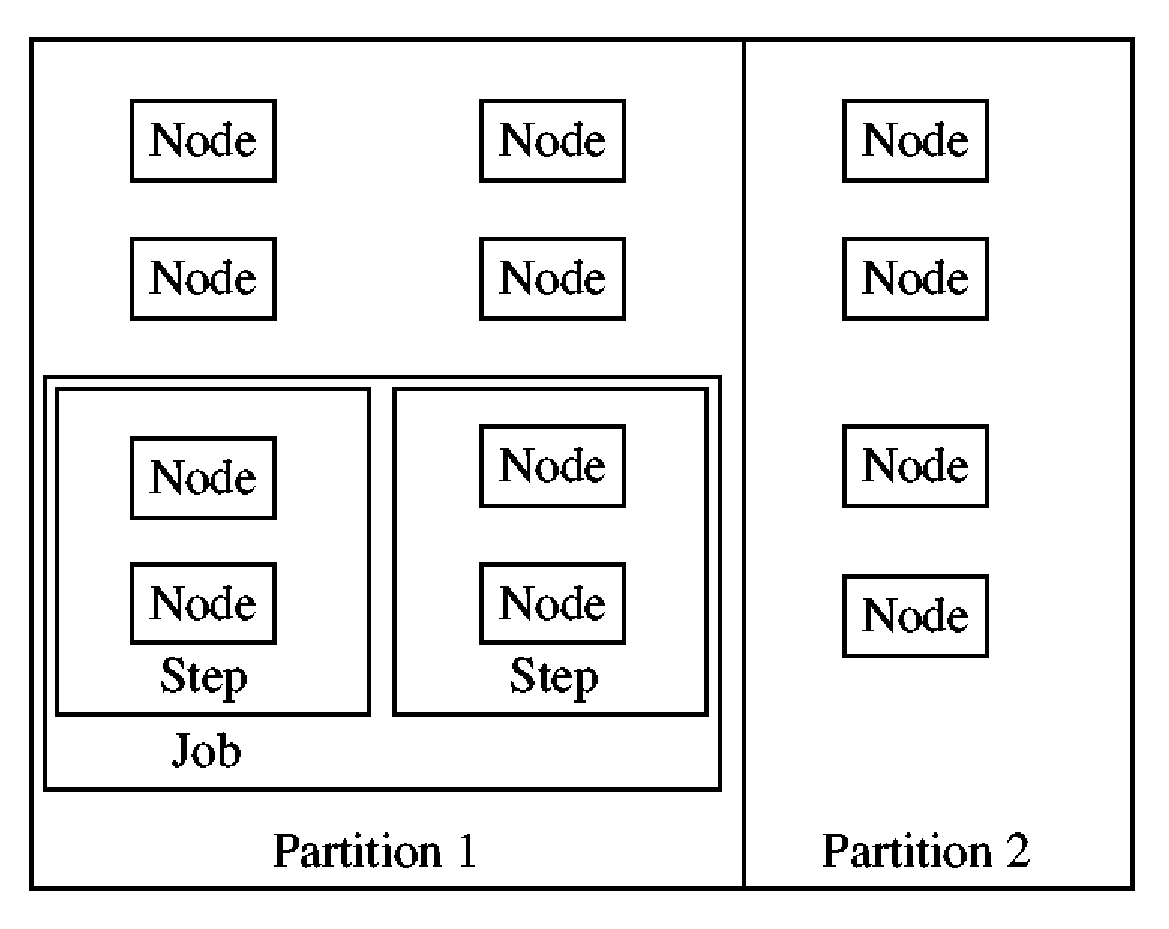
\includegraphics[width=3.32in]{../figures/entities2.eps}}
\caption{\small SLURM entities: nodes, partitions, jobs, and job steps}
\label{entities}
\end{figure}

The entities managed by SLURM are illustrated in Figure~\ref{entities} 
and include:
{\em nodes} including their processors, memory and temporary disk space,
{\em partitions} are collections of nodes with various limits and constraints,
{\em jobs} are allocations of resources assigned
to a user for a specified amount of time, and
{\em job steps} are sets of (possibly parallel) tasks within a job.
Each node must be capable of independent scheduling and job execution
\footnote{On BlueGene computers, the c-nodes can not be independently 
scheduled. Each midplane or base partition is considered a SLURM node 
with 1,024 processors. SLURM supports the execution of more than one 
job per BlueGene node.}.
Each job in the priority-ordered queue is allocated nodes within a single 
partition.
Since nodes can be in multiple partitions, one can think of them as 
general purpose queues for jobs. 

\section{Implementation}

Very high scalability was treated as a high priority for SLURM. 
More comprehensive support for smaller clusters in fact was 
added in later revisions.
For example, the initial implementation allocated whole nodes 
to jobs, in part to avoid the extra overhead of tracking individual
processors.
While allocation of entire nodes to jobs is still a recommended mode of 
operation for very large clusters, an alternate SLURM plugin provides 
resource management down the the resolution of individual processors.

The SLURM's {\tt srun} command and the daemons are extensively 
multi-threaded. 
{\tt slurmctld} also maintains independent read and 
write locks for critical data structures. 
The combination of these two features means that, 
for example, three users can get job state information at the same
time that a system administrator is modifying the time limit 
for a partition.

\begin{figure}[tcb]
\centerline{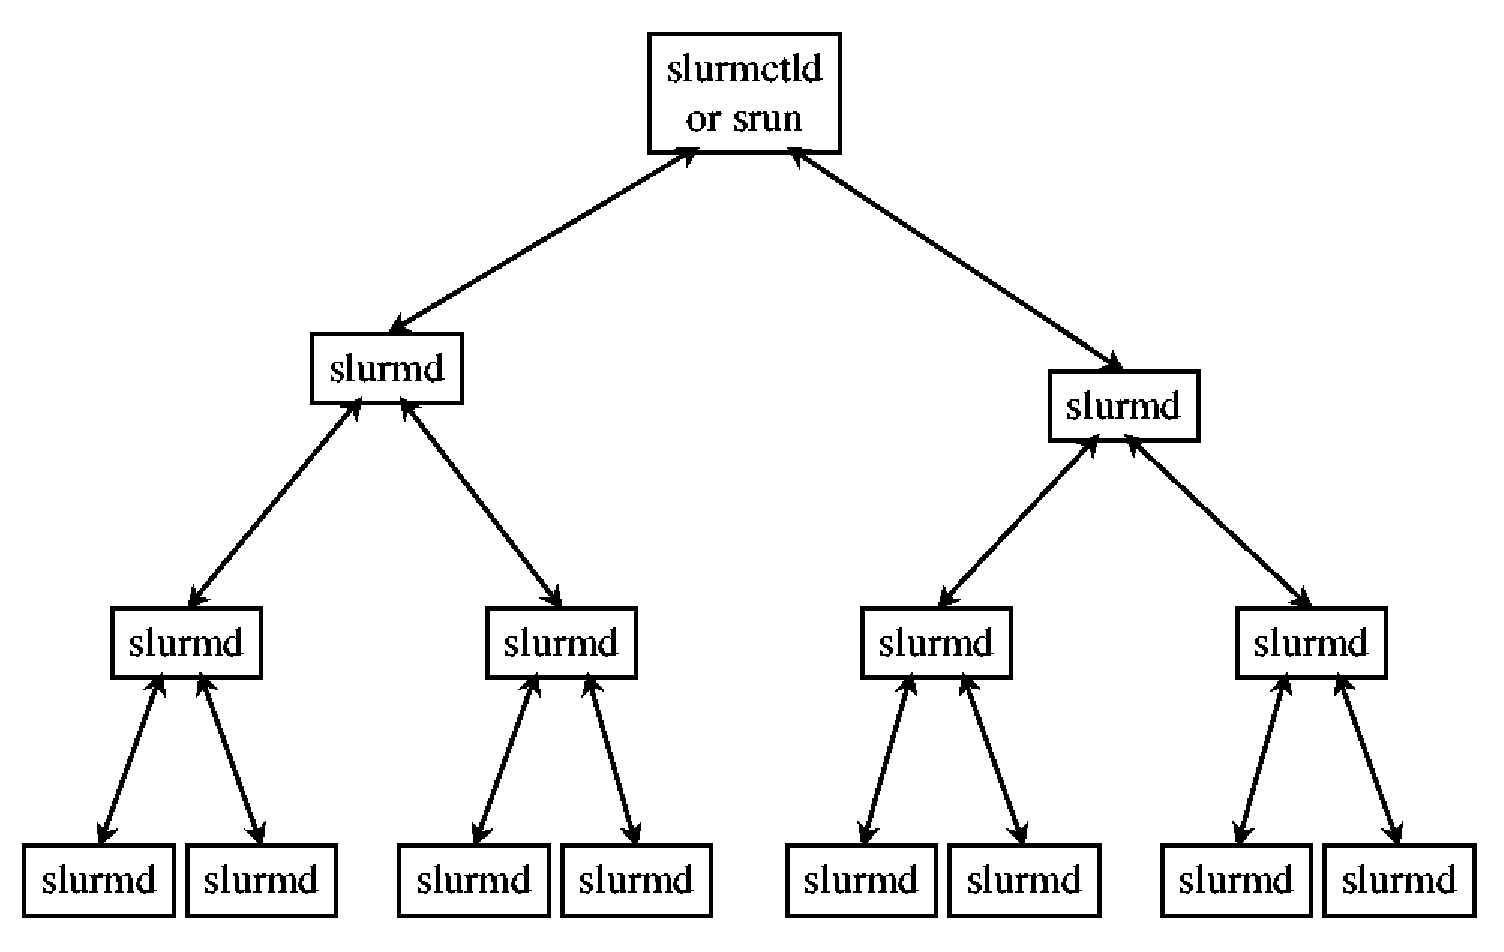
\includegraphics[width=3.32in]{../figures/comm.eps}}
\caption{\small Hierarchical SLURM communications with fanout=2}
\label{comms}
\end{figure}

Communications to large numbers of nodes are optimized in two 
ways. The programs initiating communications are multithreaded
and can process tens or even hundreds of simultaneous active 
communications. 
Second, the {\tt slurmd} daemon is designed to forward 
communications on a hierarchical basis as shown in Figure ~\ref{comms}.
For example, the initiation of tasks on 1000 nodes does not require
{\tt srun} to directly communication with all 1000 nodes. {\tt Srun}
can communicate directly with {\tt slurmd} daemons on 32 nodes
(the degree of fanout in communications is configurable). 
Each of those {\tt slurmd} will simultaneously forward the request
to {\tt slurmd} programs on another 32 nodes. 
This improves performance by distributing the communication workload.
Note that every communication is authenticated and acknowleged 
for fault-tolerance.

A number of interesting papers
~\cite{Jones2003,Kerbyson2001,Petrini2003,Phillips2003,Tsafrir2005} 
have recently been written about
the impact of system daemons and other system overhead on 
parallel job performance. This {\tt system noise} can have a 
dramatic impact upon the performance of highly parallel jobs. 
In a simplified example, consider a system daemon that run for 
one second out of every 100 seconds on every node in a cluster. 
For serial jobs this 
reduces throughput by one percent, but the impact is compounded 
on parallel computers if these daemons do not all execute concurrently. 
If the parallel program runs on 100 nodes and tries to synchronize 
every second, almost every synchronization period will include a
one second delay from the daemon running on one of the 100 nodes. 
This effectively limits job parallelism to about 50-way, orders 
of magnitude smaller than the largest systems currently available.
SLURM addresses this issue by:
\begin{itemize}
\item Making the {\tt slurmd} daemon resource requirements negligible 
\item Supporting configurations that let the {\tt slurmd} daemon sleep 
during the entire job execution period
\item If the {\tt slurmd} daemons do perform work, it is done on a 
highly synchronized fashion across all nodes
\end{itemize}
In addition, the default mode of operation is to allocate entire 
nodes with all of their processors to applications rather than 
individual processors on each node. 
This eliminates the possibility of interference between jobs, 
which could severely degrade performance of parallel applications.
Allocation of resources to the resolution of individual processors 
on each node is supported by SLURM, but this comes at a higher cost 
in terms of the data managed.
The selection of resource resolution is provided by different plugins.

Resource management of large clusters entails the processing of 
large quantities of data, both for the software and the 
system administrator.
In order to ease the burden on system administrators, SLURM 
configuration files and tools all support node naming using
numeric ranges.
For example, "linux[1-4096]" represents 4096 node names with 
a prefix of "linux" and numeric suffix from 1 to 4096. 
These naming convention permits even the largest clusters 
to be described in a configure file containing only a 
couple of dozen lines. 
State information output from various SLURM commands uses
the same convention to maintain a modest volume of output
on even large cluster. 

Extensive use is made of bitmaps to represent nodes in the cluster. 
For example, bitmaps are maintained for each unique node configuration, 
the nodes associated with each partition, nodes allocated to 
the active jobs, nodes available for use, etc. This reduces most 
scheduling operations to very rapid AND and OR operations on those bitmaps.

\section{Application Launch}

To better illustrate SLURM's operation, the execution of an 
application is detailed below and illustrated in Figure~\ref{launch}.
This example is based upon a typical configuration and the 
{\em interactive} mode, in which stdout and
stderr are displayed on the user's terminal in real time, and stdin and
signals may be forwarded from the terminal transparently to the remote
tasks.

\begin{figure}[tb]
\centerline{\includegraphics[width=3.32in]{../figures/launch.eps}}
\caption{\small SLURM Job Launch}
\label{launch}
\end{figure}

The task launch request is initiated by a user's execution of the 
{\tt srun} command. {\tt Srun} has a multitude of options to specify 
resource requirements such as minimum memory per node, minimum 
temporary disk space per node, features associated with nodes, 
partition to use, node count, task count, etc.
{\tt Srun} gets a credential to identify the user and his group 
then sends the request to {\tt slurmctld} (message 1). 

{\tt Slurmctld} authenticates the request and identifies the resources 
to be allocated using a series of bitmap operations.
First the nodes containing the appropriate resources (processors, 
memory, temporary disk space, and features) are identified through 
comparison with a node configuration table, which typically has 
a very small number of entries. 
The resulting bitmap is ANDed with the bitmap associated with the 
requested partition. 
This bitmap is ANDed with the bitmap identifying available nodes. 
The requested node and/or processor count is then satisfied from 
the nodes identified with the resulting bitmap.
This completes the job allocation process, but for interactive 
mode, a job step credential is also constructed for the allocation 
and sent to {\tt srun} in the reply (message 2).

The {\tt srun} command open sockets for task input and output then
sends the job step credential directly to the {\tt slurmd} daemons 
(message 3) in order to launch the tasks, which is acknowledged
(message 4).
Note the {\tt slurmctld} and {\tt slurmd} daemons do not directly 
communicate during the task launch operation in order to minimize the 
workload on the {\tt slurmctld}, which has to manage the entire 
cluster.

Task termination is communicated to {\tt srun} over the same 
socket used for input and output. 
When all tasks have terminated, {\tt srun} notifies {\tt slurmctld} 
of the job step termination (message 5).
{\tt Slurmctld} authenticates the request, acknowledges it 
(message 6) and sends messages to the {\tt slurmd} daemons to 
insure that all processes associated with the job have 
terminated (message 7). 
Upon receipt of job termination confirmation on each node (message 8), 
{\tt slurmctld} releases the resources for use by another job.

The full time for execution of a simple parallel application across 
a few nodes is a few milliseconds. 
The time reaches a few seconds for jobs that span thousands of 
nodes.
The times will vary with the hardware and configuration used, 
but is hardly noticeable to the user at even the largest scales.

\section{Conclusion}

SLURM has demonstrated high reliability and scalability.
It provides resource management on several clusters containing 
over 2,000 compute nodes and has emulated clusters containing 
up to 16,384 compute nodes, four times the size of of the 
largest parallel computer in use today. 
The cluster size is presently limited by the size of some SLURM 
data structures, but operation on larger systems is certainly 
feasible with minor code changes.

\raggedright
% make the bibliography
\bibliographystyle{plain}
\bibliography{project}

% make the back cover page
%\makeLLNLBackCover
\end{document}
